\chapter{One-to-many Relationships}
\label{chapter:representing-relationships}

One-to-many relationships
%such as those in an entity-relationship model,
are typically implemented in Java using the standard library collection classes.
Each object maintains a collection of the objects related to
it along a given relationship. Since one-to-many relationships are such an
important part of most data models, it is not uncommon for Java applications to
need hundreds of thousands, or even millions, of collections.
Therefore, simple decisions, like which collection class to choose,
when to create collections, and how to initialize them,
can make a big difference on memory cost.
This chapter shows how to lower memory costs when implementing
relationships with collections.
 
 \section{Choosing the Right Collection for the Task}
 \label{sec:choosing-collection}

The standard Java collection classes vary widely in terms of how much memory they use.
Not surprisingly, the more functionality a collection provides, the more
memory it consumes. Collections range from simple, highly efficient
\class{ArrayList}s to very complex
\class{ConcurrentHashMap}s, which offer sophisticated concurrent access
control at an extremely high price. 
Using overly general collections, that provide more functionality than
really needed, is a common pattern leading to excessive memory bloat.
This section looks at what to consider when choosing a collection to
represent a relationship. 

Using collections for relationships often results in many small or
empty collections.  That's because for a given relationship there are
usually lots of objects that are related to either just a few other
objects or to none at all.
When there are lots of collections with only a few entries, you need to ask  whether
the functionality of the collection you choose is worth the memory cost of that
functionality\footnote{We'll use the shorthand
\emph{relationship} to mean a one-to-many relationship, unless otherwise noted. 
We'll also use \emph{small collection} to mean a very small collection, where
the number of elements is roughly in the single digits.}

To make this discussion more concrete, let's return to the product and supplier example 
from section~\ref{sec:rarely-used}, and change it a little
 bit. Instead of only one alternate supplier, a product now may have multiple
 alternate suppliers, and each product stores a reference to a collection of alternate suppliers. An obvious choice is
 to store the alternate suppliers in a \class{HashSet}:
 \begin{shortlisting} 
class Product {
	String sku;
	String name;
	.. 
	HashSet<Supplier> alternateSuppliers;
}

class Supplier {
	String supplierName;
	String supplierAddress;
	String sku;
}
\end{shortlisting}


Suppose there are 100,000 products that each have four alternate suppliers on
average. Figure~\ref{fig:product-hashset} shows an entity-collection diagram for
the relationship between products and alternate suppliers.
 \begin{figure}
  \centering
 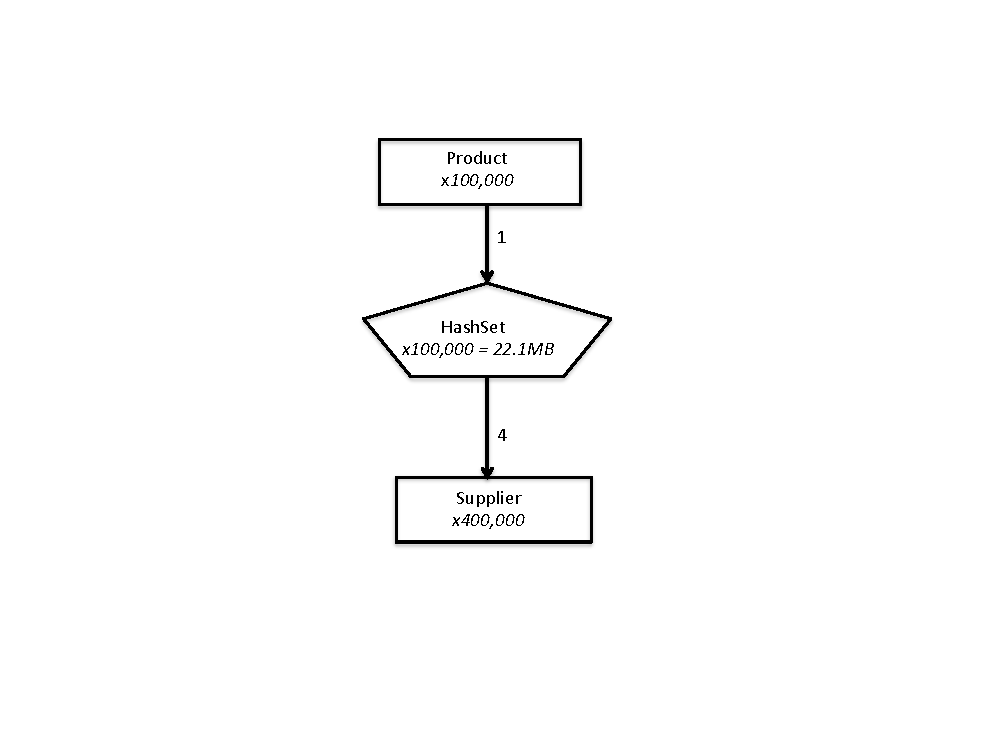
\includegraphics[width=.80\textwidth]{part1/Figures/collections/product-hashset.pdf}
 \caption{A relationship between products and alternate suppliers.
  Stored as one
  \class{HashSet} of alternate \class{Suppliers} per \class{Product}.}
  \label{fig:product-hashset}
\end{figure}


Using a \class{HashSet} for alternate suppliers turns out to be a
very costly decision. The alternate suppliers are represented by 100,000
very small \class{HashSet}s, each consuming 232 bytes, for a total cost of 22.1MB. 
This cost is all overhead.
It's hard to think of a good reason why such a heavy-weight collection should ever be used
 for storing just a few entries, and yet, this pattern is very, very common. For
 small sets, \class{ArrayList} is almost always a better choice. \class{HashSet}
 does maintain uniqueness, but enforcing uniqueness
in the data model is not always needed. Many applications
 perform this check in their loading code. If it is
important to guarantee uniqueness in the data model, it can be enforced for an
\class{ArrayList} with  little extra checking code, and usually without significant performance
 loss when sets are small.  Figure~\ref{fig:product-arraylist} shows improved memory usage with
 \class{ArrayList}. Each \class{ArrayList} incurs 80 bytes of overhead, approximately a third the size of
 a \class{HashSet}.
 \begin{figure}
  \centering
 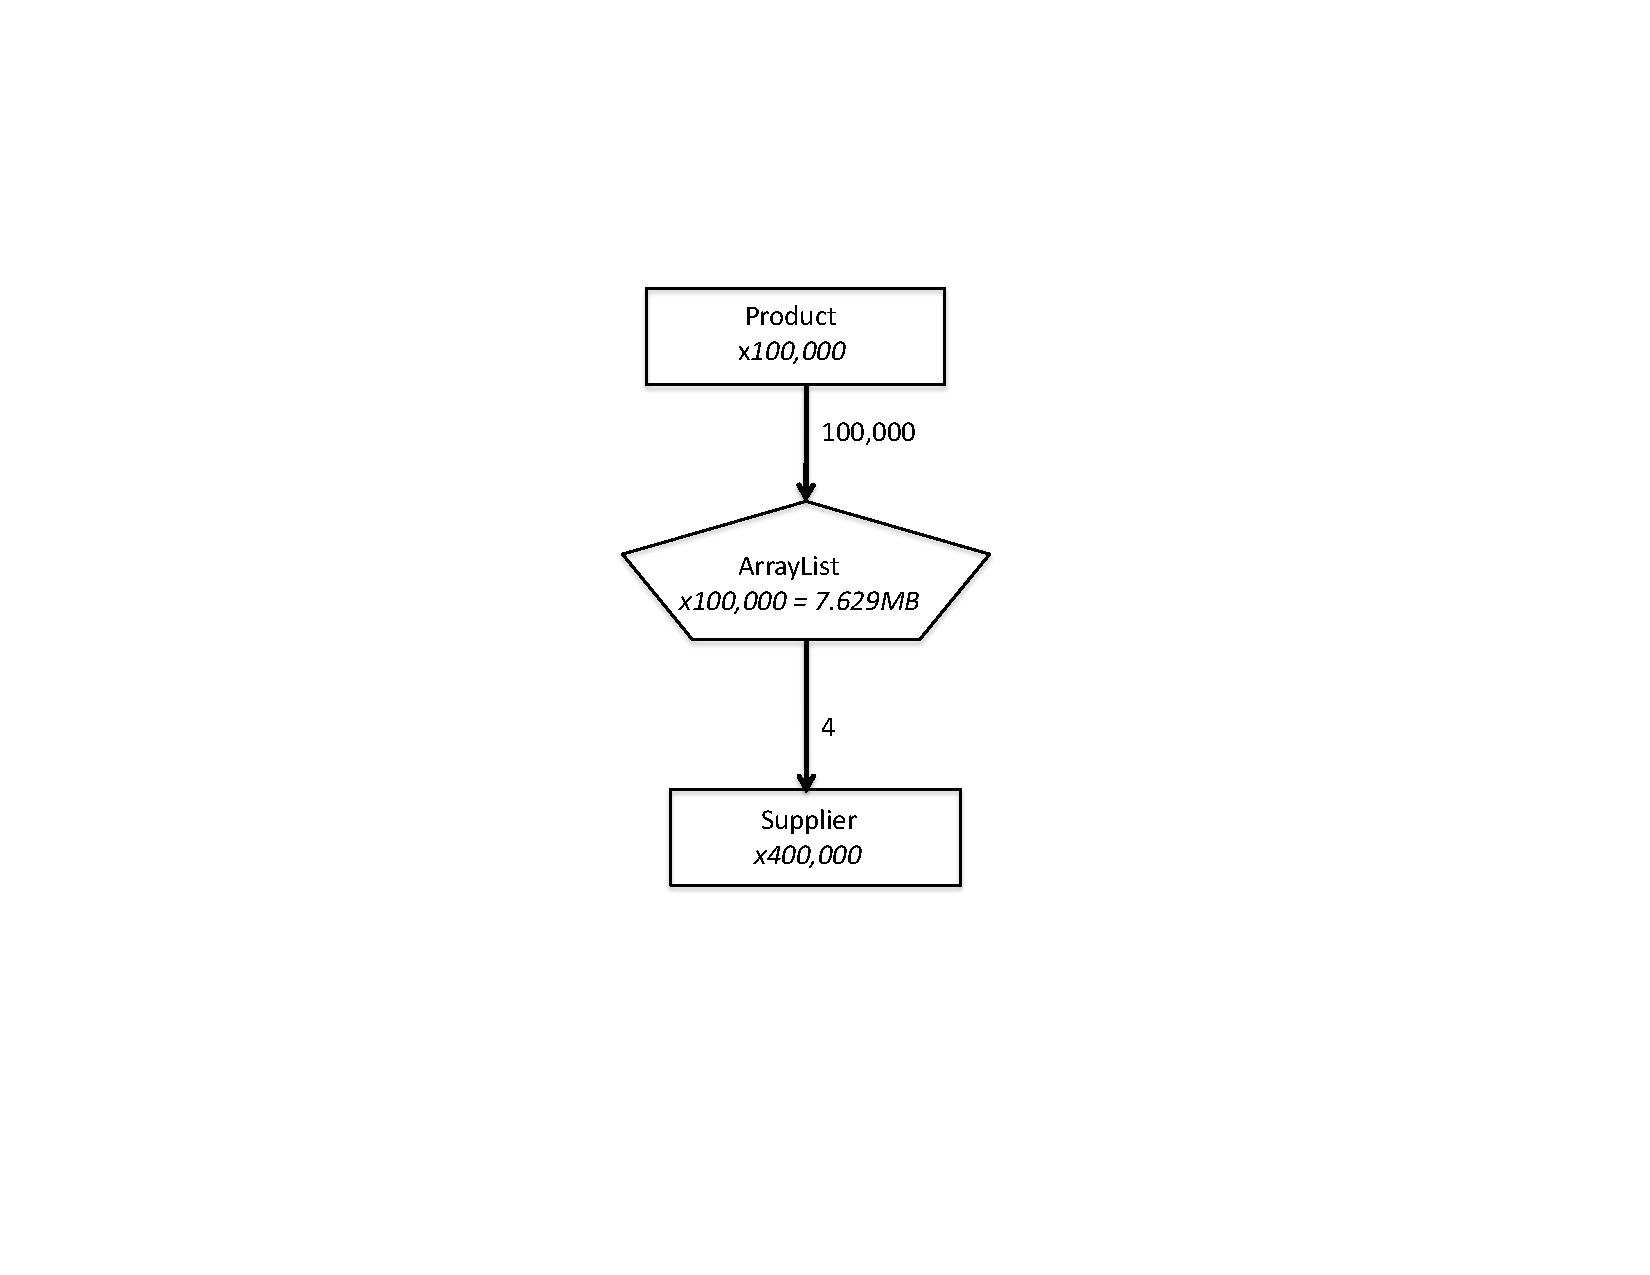
\includegraphics[width=.80\textwidth]{part1/Figures/collections/product-arraylist.pdf}
 \caption{A relationship between 100,000 products and alternate suppliers,
 where the alternate \class{Supplier}s associated with each
 \class{Product} are stored in an \class{ArrayList}.}
  \label{fig:product-arraylist}
\end{figure}
This simple change saves 14.5MB. 


\section{Inside Small Collections}
\label{sec:collectioncost}
Let's look inside a \class{HashSet} to see why it is so much bigger than an
\class{ArrayList}.
The structure of a \class{HashSet} is shown in
Figure~\ref{fig:inside-hashset}. All
collections have a similar basic structure: a wrapper
which remains stable, and an internal structure that changes as entries are
added and removed.

The standard library designers implemented
\class{HashSet} by delegating its work to a degenerate \class{HashMap},
that is, one with keys but no values.
The \class{HashSet} object is therefore just a wrapper, and it points to a
\class{HashMap} wrapper. All collections have
wrapper objects, but a \class{HashSet} has two of them. 
%Together they incur a fixed cost of 56 bytes.

\class{HashMap} itself uses a \emph{chaining}
design. Its internal structure is an array of hash buckets, with initial size of
16 by default.  Each bucket is a linked
list of \class{HashMap\$Entry} objects. Each entry object
points to an element of the user's data, in other words, to a key and value.

 \begin{figure}
  \centering
 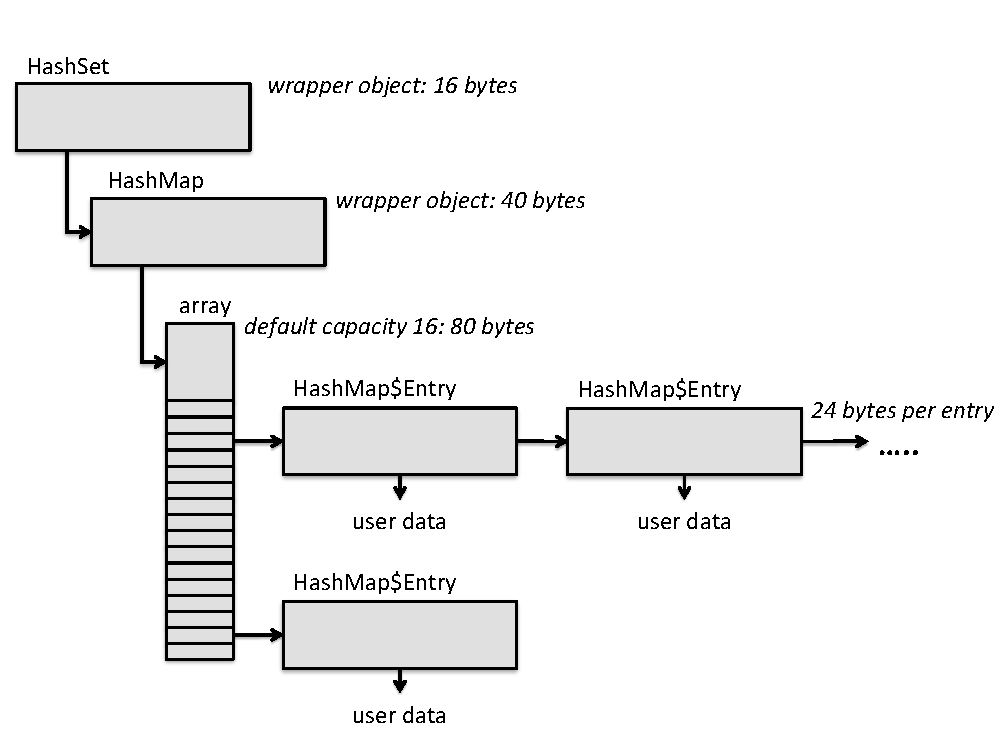
\includegraphics[width=.80\textwidth]{part1/Figures/collections/inside-hashset.pdf}
  \caption{A look inside a \class{HashSet}. Shown with 3
  entries.}
  \label{fig:inside-hashset}
\end{figure}

In contrast, \class{ArrayList} is a simpler structure, as shown in
Figure~\ref{fig:inside-arraylist}. It's an expandable array,
consisting of a wrapper object and an array.  The array points directly to the
user data. The array has an initial size of 10 by default.  As a result of its
simpler design \class{ArrayList} has a smaller fixed cost and a smaller
variable cost than \class{HashSet}.

The fixed cost is the memory needed before any entries are added.
For a \class{HashSet} the fixed cost consists of two wrapper objects, taking 56 bytes, plus
the array's \jre overhead and 16 slots, bringing the total to 136 bytes. We are including the
array's empty slots as a fixed cost since they are allocated right from the start
\footnote{Once a collection grows beyond its initial size, we'll treat
treat excess capacity as a variable cost, as we discuss in the next chapter.
%This is because growth policies allocate excess capacity
%in proportion to the size of the collection
}
\footnote{\class{HashSet} often has another
fixed cost, not shown in our figures.  The first time you iterate over
the set, a 16-byte \class{HashMap\$KeySet} is created and retained for the lifetime of
the set.}.
The fixed cost of an \class{ArrayList} is considerably
lower, a total of 80 bytes. That includes its wrapper object and default
10-element array. Fixed costs matter most in
small collections. As collections grow they become less significant.

A \class{HashSet} maintains a \class{HashMap\$Entry} object for 
each entry, at 24 bytes each. This is its
variable cost, that is, the incremental cost of storing an
entry. It is much higher than that of an \class{ArrayList}, which
use a 4-byte array slot to point to each entry.
A lower variable cost means that \class{ArrayList} scales much
better than \class{HashSet} for large collections. The variable cost also
adds up for small collections, whenever you have a lot of instances of them.  
%Note that we treat the variable cost of a small \class{ArrayList} to be 0,
% since we've already counted the 10 initial slots in the fixed cost.
 \begin{figure}
  \centering
 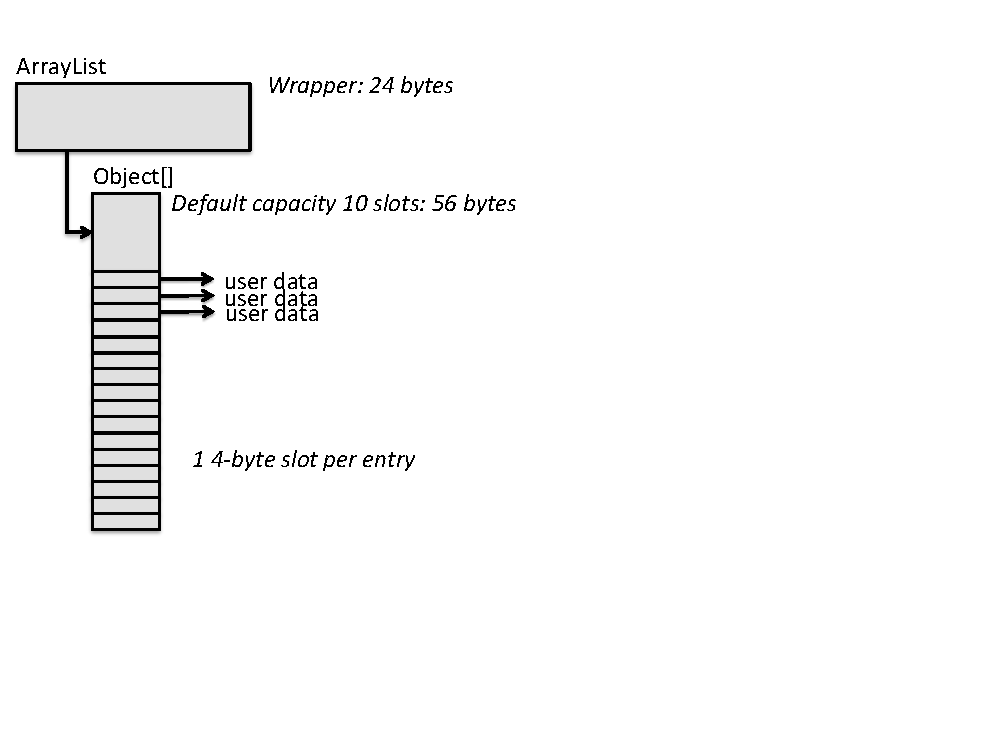
\includegraphics[width=.80\textwidth]{part1/Figures/collections/inside-arraylist.pdf}
 \caption{Inside an \class{ArrayList}. Shown with three
 entries and default capacity. \class{ArrayList} has a relatively low
 fixed overhead, and is scalable.}
  \label{fig:inside-arraylist}
\end{figure}
 

In summary, why does \class{HashSet} take more space than \class{ArrayList}?
We can see a number of reasons. Some of the extra cost is because of
additional functionality, such as providing uniqueness checking and entry
removal, in constant time.
\class{HashSet} is also optimized for performance, and sacrifices memory 
under the assumption that \class{HashSet}s will contain a large number of
elements. The decision
to reuse the more general \class{HashMap} code adds to the memory needed,
especially the fixed cost. Other extra costs
are due to unavoidable Java overhead.
Our guess is that the collection class developers would be surprised by the relationship usage
pattern that results in hundreds of thousands of small \class{HashSets}. 
%Why bother
%implementing expandable structures and clever hashing algorithms for only a few
% entries? 
This mismatch between collection implementation and usage is 
a leading cause of memory bloat. 
%The overhead cost of a \class{HashSet} is
%remarkably high. Creating many small collections multiplies this basic
% infrastructure cost, which is all overhead, filling the heap. 

%The fact that \class{HashSet} delegates to \class{HashMap} inflates its fixed
%cost in two ways: the cost of the extra wrapper object, and the cost of fields
%in the \class{HashMap} that aren't needed when it's used as a set. 
%Note that since the \class{HashMap\$Entry} class is designed for
%a \class{HashMap}, its value field is not used.

 
%Let's look now at some additional choices for small collections.
Table~\ref{tab:small-collections-default} compares the memory costs of four
common classes from the standard libraries.
The table shows bytes needed when each collection contains just a few
entries, plus fixed and variable costs for computing the memory needed for small sizes
in general. All have been allocated with default capacity.
%and the default size when the collection is just allocated without entries, and
% any additional entry cost. 
These costs have been calculated based on the \oracle \jre,
using the techniques described in Chapter~\ref{chapter:delegation}.
%The various other Java standard
%library implementations in circulation have costs
%similar to these. 
You can calculate costs for similar classes using the same methodology.
\autoref{chapter:jre-comparison} has more information about additional classes
and \jre platforms.


\begin{table}
\centering
 		\begin{tabular}{l||r||r||rrl}
 		\toprule
	 	 Collection & with 1 entry & with 4 entries & \multicolumn{3}{c}{with n entries}\\
	 	 & & & fixed & variable & comments \\
	 	 \midrule
	 	ArrayList & 80 & 80 & 80 & 0 & for n in 0..10 \\
 		HashMap & 144 & 216 & 120 & 24 & for n in 0..12 \\
 		HashSet & 160 & 232 & 136 & 24 & for n in 0..12 \\
 		LinkedList & 72 & 144 & 48 & 24 & for any n \\
	 	\bottomrule
	 	\end{tabular}
	 	
	\caption{Cost of some common collections when they
	contain very few entries and are allocated with default capacity. Variable
	cost is the cost per entry, above the fixed cost of the collection. Costs apply only within the specified
	range.}
	\label{tab:small-collections-default}
\end{table}

\begin{figure}
  \centering
 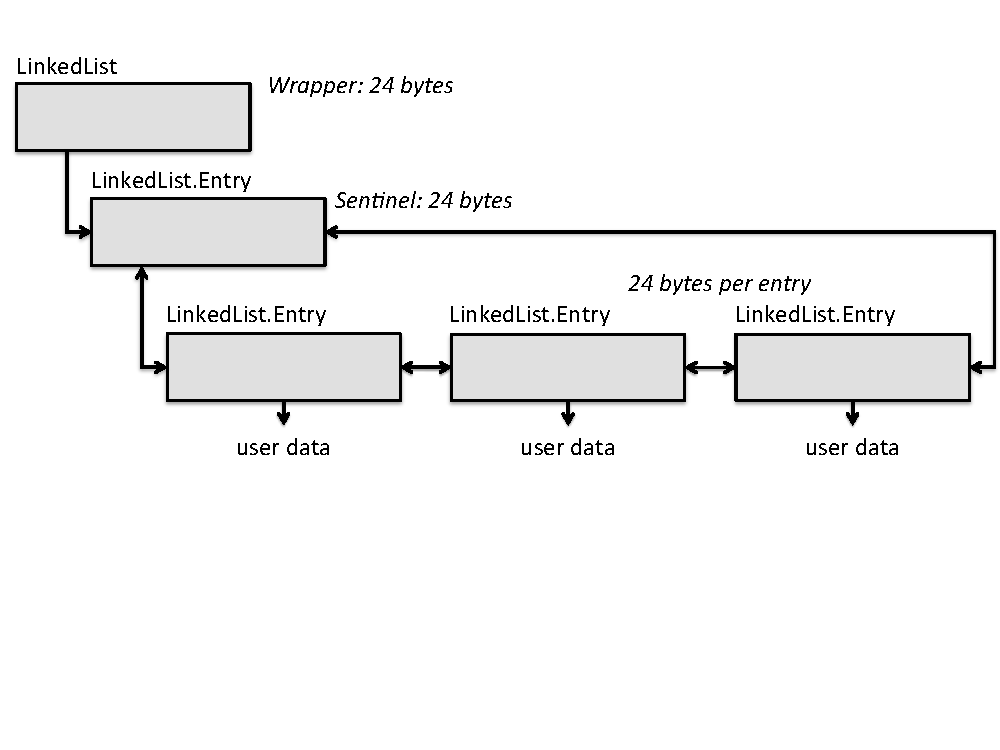
\includegraphics[width=.80\textwidth]{part1/Figures/collections/inside-linkedlist.pdf}
 \caption{A look inside a \class{LinkedList}. Shown with 3
  entries.}
  \label{fig:inside-linkedlist}
\end{figure}

Let's now look at one more choice, \class{LinkedList}, useful when ordering is
needed and there are frequent insertions or deletions.
\autoref{fig:inside-linkedlist} shows its internal structure. A
\class{LinkedList} always has one wrapper object, plus a dummy entry object that
acts as an end-of-list sentinel, presumably for performance reasons. The total
fixed cost is 48 bytes.
\class{LinkedList}, just like \class{HashSet}, \class{HashMap}, and
\class{TreeMap}, is an \emph{entry-based} collection, where an internal entry object
is allocated for each element in the collection. Each \class{LinkedList.Entry}
requires 24 bytes, the variable cost of the collection. Entry-based collections
have higher variable costs than \emph{array-based} collections,
such as \class{ArrayList}, which point directly to the user data from array
slots.
The combination of fixed and variable costs can make \class{LinkedList} an
expensive choice even at small sizes.  From
\autoref{tab:small-collections-default} we can see that a 4-element
\class{LinkedList} is much larger than the equivalent \class{ArrayList}. Again, for such
small collections it's worth
asking what the performance gains
are in practice, compared to an array-based representation.  In the next chapter
we'll look at a few examples of array-based maps and sets from some open source
frameworks, in the context of larger collections. A few of these are appropriate
for small collections as well.




\begin{table}
\centering
 		\begin{tabular}{l||rr||rr}
 		\toprule
	 	 Collection & \multicolumn{2}{c}{with 1 entry} & \multicolumn{2}{c}{with 4 entries}\\
	 	 & default & minimum & default & minimum \\
	 	 \midrule
	 	ArrayList & 80 & 40 & 80 & 56 \\
 		HashMap & 144 & 80 & 216 & 184 \\
  		HashSet & 160 & 96 & 232 & 200 \\
 	 	\bottomrule
 	 	\end{tabular}
	\caption{The effect of capacity on the cost of some small collections,
	comparing the default capacity with the minimum to accomodate the number of entries.
	For \class{HashMap} and \class{HashSet}, 1 entry requires a capacity of 2, and 4 entries requires a capacity
	of 8.}
	\label{tab:small-collections-minimum-samples}
\end{table}

\begin{table}
\centering
 		\begin{tabular}{l||rrl}
 		\toprule
	 	 Collection & \multicolumn{3}{c}{with n entries}\\
	 	 & fixed & variable & comments \\
	 	 \midrule
	 	ArrayList & 36 \footnotemark[1] & 4 & for any n \\
	 	\midrule
 		HashMap &  64 & 24 & capacity = 2, holds up to 1 \\
 		        &  72 & 24 & capacity = 4, holds up to 3 \\
 		        &  88 & 24 & capacity = 8, holds up to 6 \\
 		\midrule
 		HashSet &  80 & 24 & capacity = 2, holds up to 1\\
 		        &  88 & 24 & capacity = 4, holds up to 3 \\
		        &  104 & 24 & capacity = 8, holds up to 6 \\
	 	\bottomrule
 	 	\end{tabular}
	\caption{Fixed and variable costs of some common collection classes when capacity is set
	to the minimum to accomodate the number of entries.}
	\label{tab:small-collections-minimum-fixed-var}
\end{table}

\footnotetext[1]{Round total cost up to nearest 8 bytes.}

\section{Properly Sizing Collections}
\label{sec:proper-size}

Many collection classes, such as \class{ArrayList}, \class{HashMap} and
\class{HashSet}, use arrays in their implementations. When the array becomes
full, a larger array is allocated and the contents are copied into the new array.
Since allocation and copying can be expensive, these arrays are
allocated with extra capacity, to avoid paying these growth costs too
often. 
%This is why
By default, the initial capacity of an \class{ArrayList} is 10, and the capacity
increases by 50\% whenever the array is reallocated.
The capacity of a \class{HashMap} or \class{HashSet}
starts at 16 by default, and grows by a factor of 2 when the collection becomes
more than 75\% full.

These policies trade space
for time, on the assumption that collections always grow.
However, many applications have relationships with
hundreds of thousands of collections that do not grow once the data has
been loaded. Most may never contain more than a few elements. 
In these cases, the empty array slots can add up to a
significant bloat problem, with nothing gained in performance. 
The same holds true for larger collections that stop growing. 
%,unless you take explicit action.

Fortunately, it is often possible to right-size collections at creation
time, by specifying an initial capacity. For example, if you know that an
\class{ArrayList} has a maximum size of $x$, which is less than the default
size, then you can set its initial capacity to $x$ when calling its constructor. On the
other hand, the standard collections do not give you much control over their
growth policies. So if you are wrong and the \class{ArrayList} grows bigger than
$x$, extra capacity will be allocated, which may be worse than just taking the
default. 
 
For an \class{ArrayList}, another approach is to call its \code{trimToSize}
method, which shrinks the array by eliminating the extra growth space. 
Since trimming reallocates and copies the array, it is expensive to call
\code{trimToSize} while a collection is still growing. Trimming is
appropriate after a collection is fully populated. In 
applications where the data has a build phase followed by a use phase,
the \class{ArrayList}s can be trimmed between these two phases.
%so that the cost of reallocation and copying is paid only once.
 
Returning to the example of the relationship between products and alternate
suppliers, the \class{ArrayList}s in Figure~\ref{fig:product-arraylist} have
been initialized with default capacity. If we assume that the the relationship
is built in one phase and used in another phase, then it is possible to trim the
\class{ArrayList}s after the first phase. This should save quite a bit of
space, since there are 100,000 \class{ArrayList}s with four entries on
average. In fact, trimming these
\class{ArrayList}s saves 2.3MB, or another 30\%, as shown in
Figure~\ref{fig:trimmed-product}. 

\begin{figure}
  \centering
 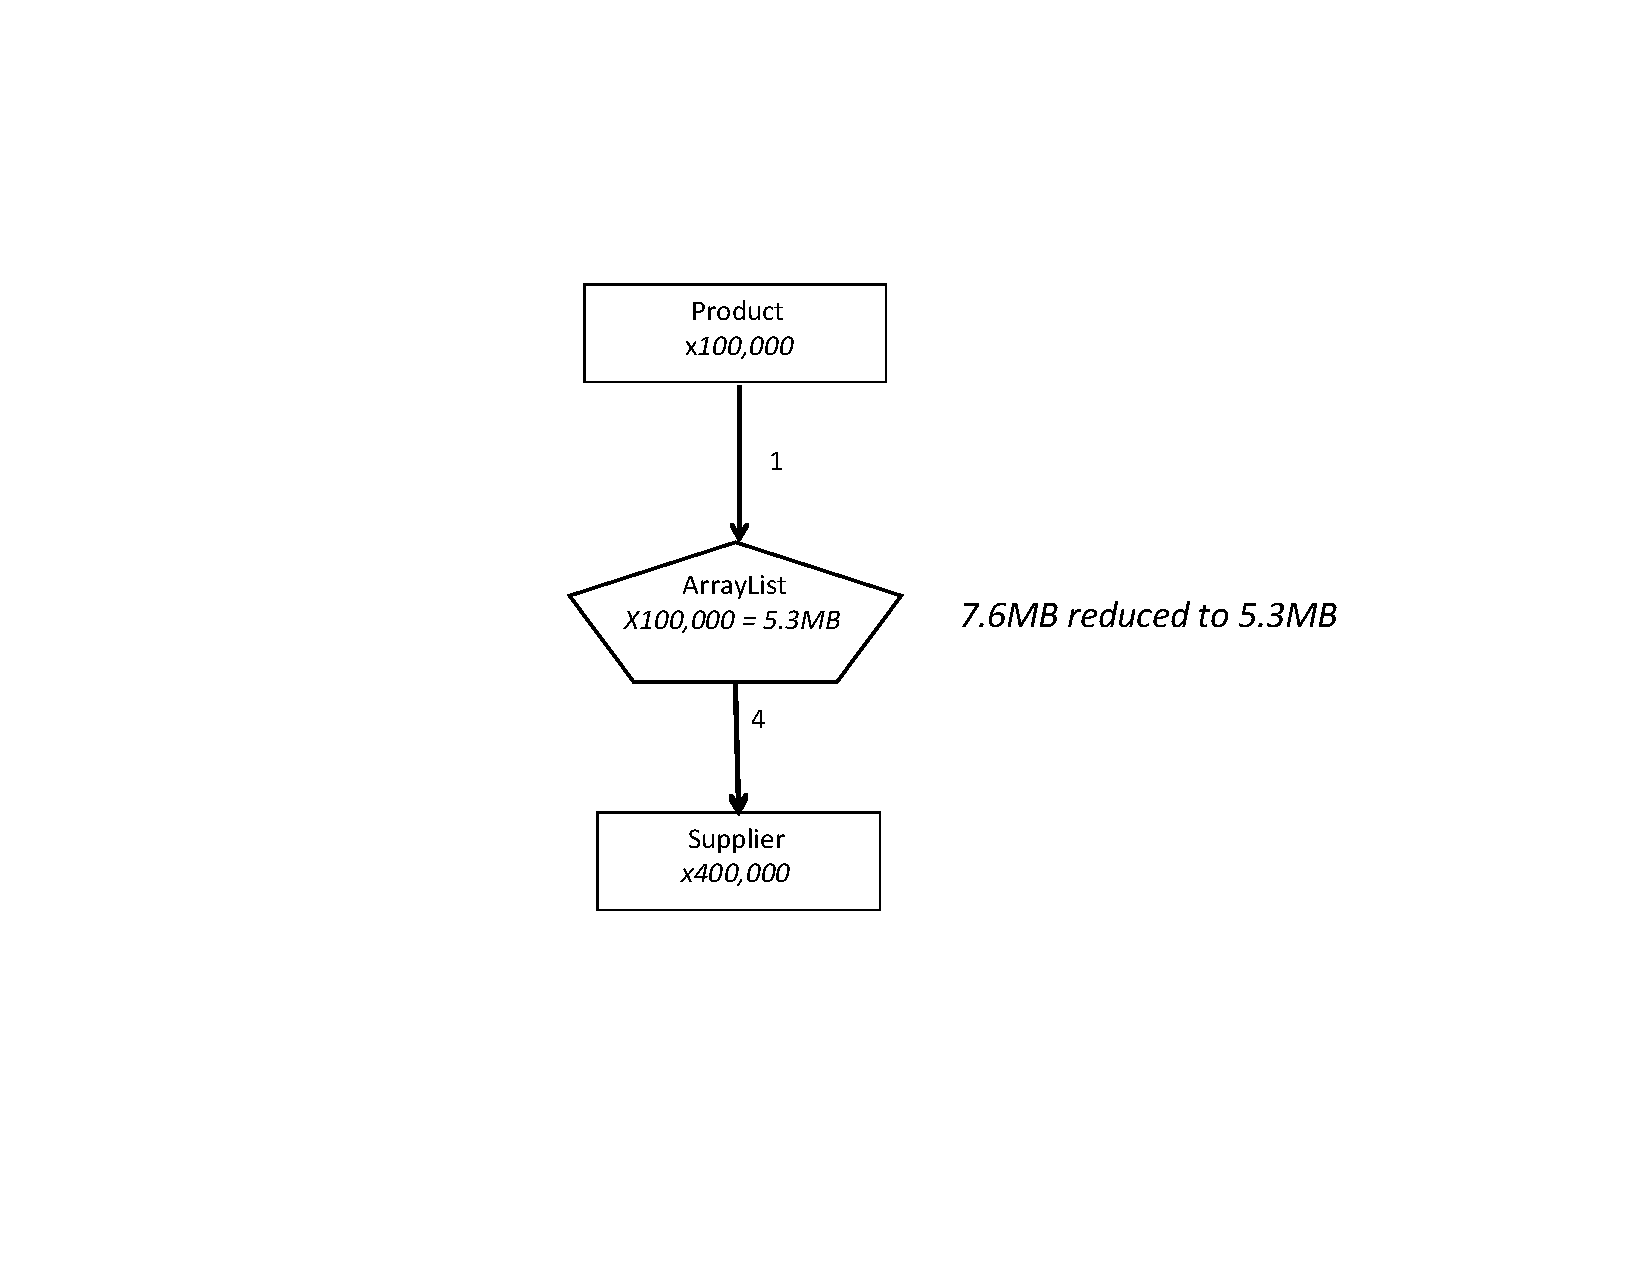
\includegraphics[width=.80\textwidth]{part1/Figures/collections/trimmed-product.pdf}
 \caption{The relationship between \class{Product}s and \class{Supplier}s after
 all of the
 \class{ArrayLists} have been trimmed by calling the \code{trimToSize} method.}
  \label{fig:trimmed-product}
\end{figure}
 
\class{HashSet}s and \class{HashMap}s do not have \code{trimToSize}
methods, but it is possible to set their initial capacity at construction time.
The capacity is actually not the number of elements the collection is
expected to hold. It specifies instead the number of hash buckets, that is, the
number of slots in the array. It is automatically rounded up to the
nearest power of two. Hash-based collections always require some excess capacity to reduce the
likelihood of collisions. In addition, if the collection does grow and the
array needs to be reallocated, there will be the expense of
rehashing the entries. The load factor, by default .75, determines the
maximum number of elements in the collection, relative to the size of the array,
before a larger array needs to be allocated. Therefore, it is important to take
the load factor into account when setting capacity. For example, a default
\class{HashMap} with capacity of 16 can hold a maximum of 12 elements
before needing to allocate a larger array. 
%so that you leave enough headroom

\autoref{tab:small-collections-minimum-samples} gives a sense of the savings you can achieve
for some common small collections by setting the capacity to the minimum.
\autoref{tab:small-collections-minimum-fixed-var} shows the breakdown into fixed and variable costs for some
minimally-sized collections. You can see, compared to \autoref{tab:small-collections-default}, 
how minimal sizing reduces the fixed cost.

An \class{ArrayList}, \class{HashMap}, or \class{HashSet}
will not automatically reduce the size of its array when elements are removed,
or when the collection is cleared.

%However, before changing the initial capacity, you should
%ask yourself whether using a \class{HashSet} or \class{HashMap} is a
%wise decision in the first place. If you are going to end up with many
%collections with fewer than 16 elements, perhaps there is a more
% memory-efficient solution, like \class{ArrayList}.
  
%A \class{LinkedList} is another alternative for small collections, and are
%better than \class{ArrayLists} if the collections are changing a lot. The
%24 byte per-entry cost is larger, but there is no element array, and only one
%extra entry, which is a sentinal.

\section{Avoiding Empty Collections}
\label{sec:empty-collections}

Maintaining a large number of empty collections is another common problem that
leads to memory bloat. Empty collection problems are generally caused by eager
initialization, that is, by allocating collections before they are actually
needed. You might think that eager initialization would not be a big
problem, since entries will be added eventually. However, it's common to
find large numbers of collections that remain empty throughout an execution.

Making matters worse, the standard collections
allocate their internal objects in an eager fashion. For example,
\class{ArrayList} allocates its internal array before any
entries are inserted, and \class{LinkedList} always allocates a sentinel
entry. As a result, every empty collection takes two or more objects, as shown
in \autoref{fig:inside-empty}.
This is true even if you allocate the collection with the minimum possible
capacity.
Therefore, the smallest empty collections are still quite large. For example,
a zero-capacity \class{ArrayList} requires 40 bytes.
\autoref{tab:empty-collection-costs} shows the sizes for some common collection classes
when empty. 

%a zero-sized \class{ArrayList}
%consumes 40 bytes, the smallest \class{HashMap} takes 64 bytes, and the
% smallest \class{HashSet} takes 80 bytes. Table 

%A quick look inside the empty collections show that they
%are not all that empty! 


 \begin{figure}
  \centering
 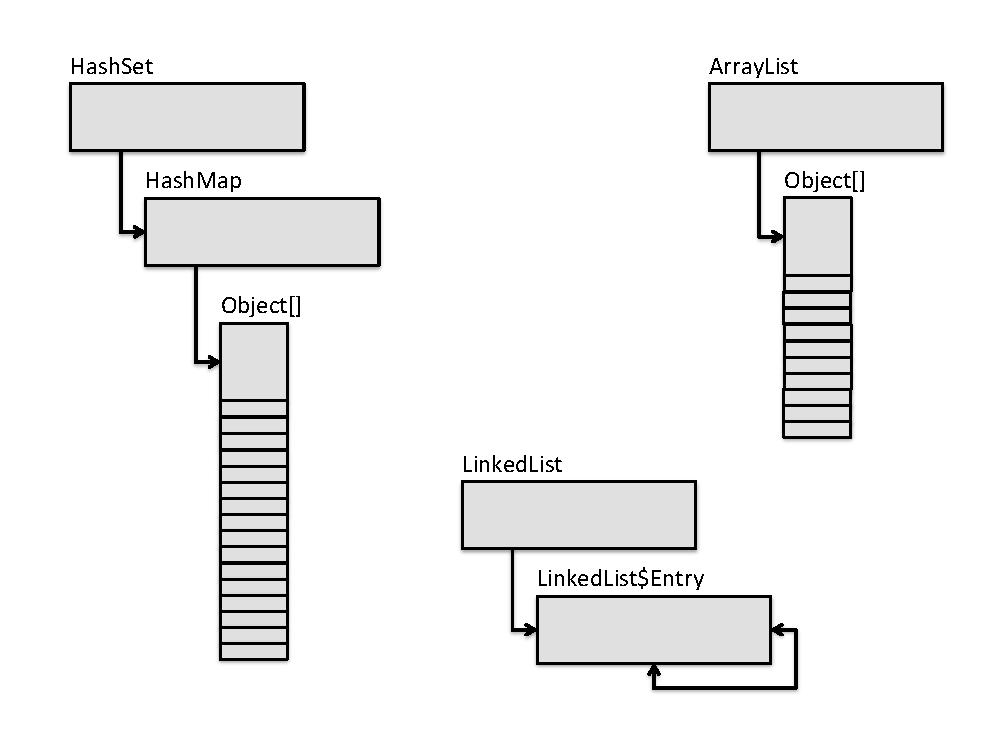
\includegraphics[width=.80\textwidth]{part1/Figures/collections/inside-empty.pdf}
  \caption{The internal structure of three empty collections. Each
  requires at least two objects, before any entries are added.}
  \label{fig:inside-empty}
\end{figure}

\begin{table}
\centering
 		\begin{tabular}{lcc}
 		\toprule
	 	 Collection & \multicolumn{2}{c}{Size in bytes} \\
	 	 & default capacity & minimum capacity \\
	 	 \midrule
	 	ArrayList & 80 & 40 \\
 		LinkedList & 48 & 48 \\
 		HashMap & 120 & 56 \\
 		HashSet & 136 & 72 \\
	 	\bottomrule
	 	\end{tabular}
	\caption{Size of empty collections, for some common
	collection classes.
	Empty collections require a lot of space, even when initialized to the smallest
	possible capacity.}
	\label{tab:empty-collection-costs}
\end{table}

\paragraph{Example} Suppose the relationship
in Figure~\ref{fig:trimmed-product} is initialized by the code:
%\begin{shortlisting}
%List<Product> products;
%int numProducts;
%..
%public void initAlternateSupplierRelationship() {
%	..
%	for (int i = 0; i < numProducts; i++) {
%    	Product product = products.get(i);
%		product.alternateSuppliers = 
%                           new ArrayList<Supplier>();
%    }
%}
%\end{shortlisting}

\begin{shortlisting} 
class Product {
	.. 
	ArrayList<Supplier> alternateSuppliers;
	..
	public Product() {
		..
		// Allocate the collection in advance
		alternateSuppliers = new ArrayList<Suppliers>();
		..
	}
}
\end{shortlisting}
Initially, each product allocates an empty \class{ArrayList} for alternate
suppliers, so there are 100,000 empty \class{ArrayLists} before any
\class{Supplier}s are inserted. As the alternate suppliers are populated, many
of these \class{ArrayLists} will become non-empty, but it is likely that a good
number of products have no alternate suppliers. If 25\% of the products have no
alternate suppliers, there will be 25,000 empty \class{ArrayLists}, which consume
about 1MB even after calling \code{trimToSize}.
Figure~\ref{fig:empty-array} shows the entity-collection
diagram after removing 25,000 empty alternate supplier \class{ArrayList}s.
The diagram now shows only 75,000 alternate supplier \class{ArrayList}s,
since there are no more empty \class{ArrayList}s. We therefore adjust the
average fanout in and out of \class{ArrayList} to .75 and 5.33, respectively.
\begin{figure}
  \centering
 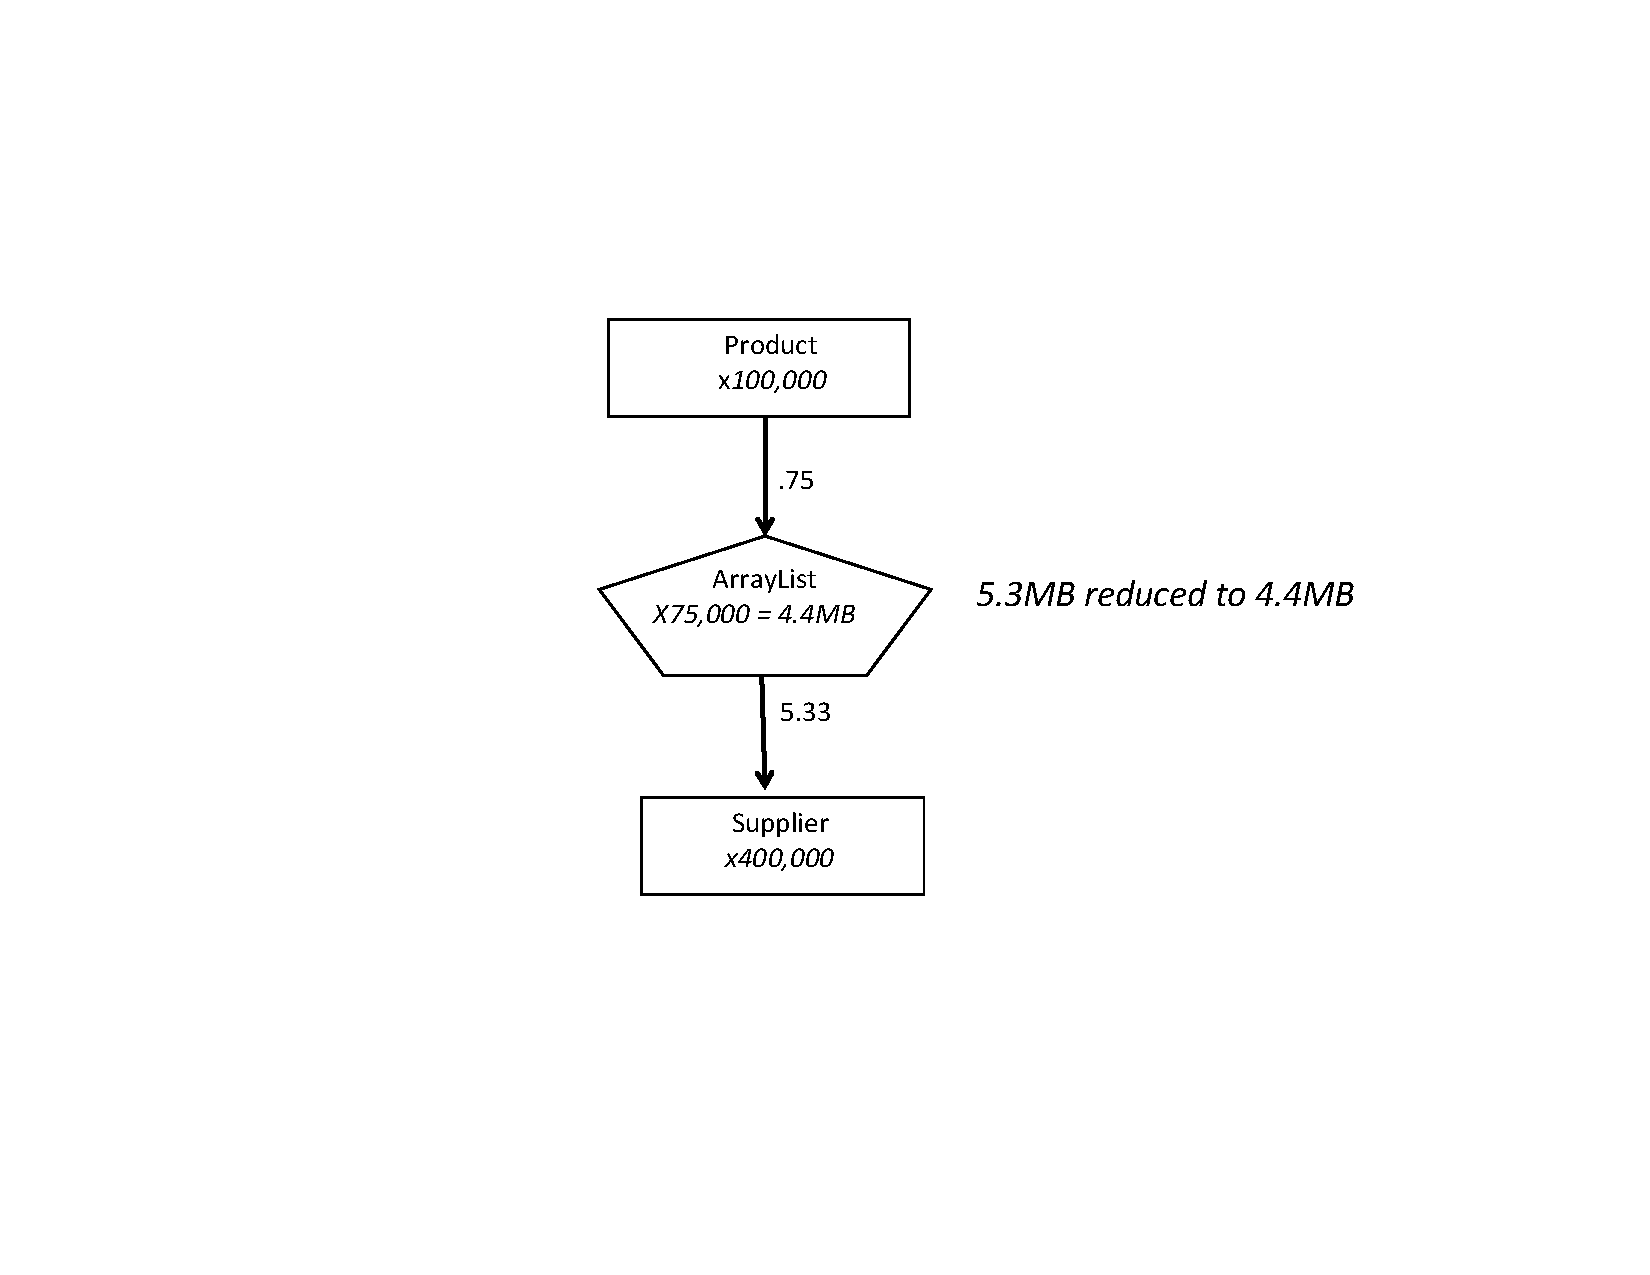
\includegraphics[width=.80\textwidth]{part1/Figures/collections/empty-product.pdf}
 \caption{The relationship between \class{Product}s and \class{Supplier}s,
  with no empty \class{ArrayLists}.}
  \label{fig:empty-array}
\end{figure}
 
 \paragraph{Lazy allocation} Delaying allocation is the way to
 avoid creating lots of empty collections.
 That is, instead of initializing all of the collections that you think you
 may need, allocate them on demand. 
 One approach is simply to leave collection fields null
 until needed. However, this requires extra checking code whenever you
 access these fields, to avoid \code{NullPointerException}s.
 
For many applications, the abstract
\class{Collections} class provides a better solution. You can initialize
collection fields to point to shared, immutable empty collections, using the
static methods \code{emptySet()}, \code{emptyList()}, and \code{emptyMap()}
\footnote{Static constants EMPTY\_SET, EMPTY\_LIST, and EMPTY\_MAP provide a similar capability,
without the type safety of generics.}.
The following code
maps all products to a single, immutable, empty list of suppliers, so that no
empty \class{ArrayLists} are created:

\begin{shortlisting}
class Product {
	.. 
	List<Supplier> alternateSuppliers;
	..
	public Product() {
		..
		// Initialize to a shared, static collection
		alternateSuppliers = Collections.emptyList();
		..
	}
}
\end{shortlisting}

This initialization avoids the need to check whether an \class{ArrayList}
exists at every use. The size method, iterators, and other access functions
work as in any other collection.
However, you have to be careful not to let any references to these static empty
collections escape their immediate context. If you do give out a reference, 
then there is no way to update this reference once an actual collection is
allocated. Instead, you can provide access and update methods to the relationship,
so that the implementation remains hidden.
You will also need to code to interfaces, delaying the use of a concrete class
until a collections is actually allocated. In this example, \code{Product}
declares a \code{List} of suppliers, so that it can point to either the shared
empty list, or to an \class{ArrayList} once it's populated.
This is, of course, a good practice in general, so that the implementation can
be easily changed later.

If lazy allocation is not a good option for your application, then
right-sizing collections, at initialization time or after loading is
completed, will still make a difference for empty collections.

%\section{Fixed Size Collections}
%
%Java collections can grow to be
%arbitrarily big, but this functionality comes at a cost.
%Collections include wrapper objects, and 
%may be sized with extra growth room. If
%you know that the size of a collection is fixed, having the ability to expand
%the collection is unnecessary, and it is better to choose a cheaper
% alternative.
%In fact, often you can use a
%simple Java array, and not use a collection at all.  
%
%In our example, alternate suppliers are stored in an
% \class{ArrayList}, which inside is a
%wrapper pointing to an array of \class{Suppliers}.  If we assume that
%every product has at most four alternate suppliers, then  it isn't 
%necessary to store these in an \class{ArrayList} --- a simple array will do.
%Eliminating the \class{ArrayList} object removes 24 bytes per
%product, but we have to add 4 bytes to each \class{Product} to store the number
%of alternate suppliers. The total savings is 1.43MB for 75,000 products:
%\begin{shortlisting} 
%class Product {
%	String sku;
%	String name;
%	.. 
%	int numAlternateSuppliers;
%	Supplier[4] alternateSuppliers;
%}
%\end{shortlisting}
 

%\begin{figure}
 % \centering
% 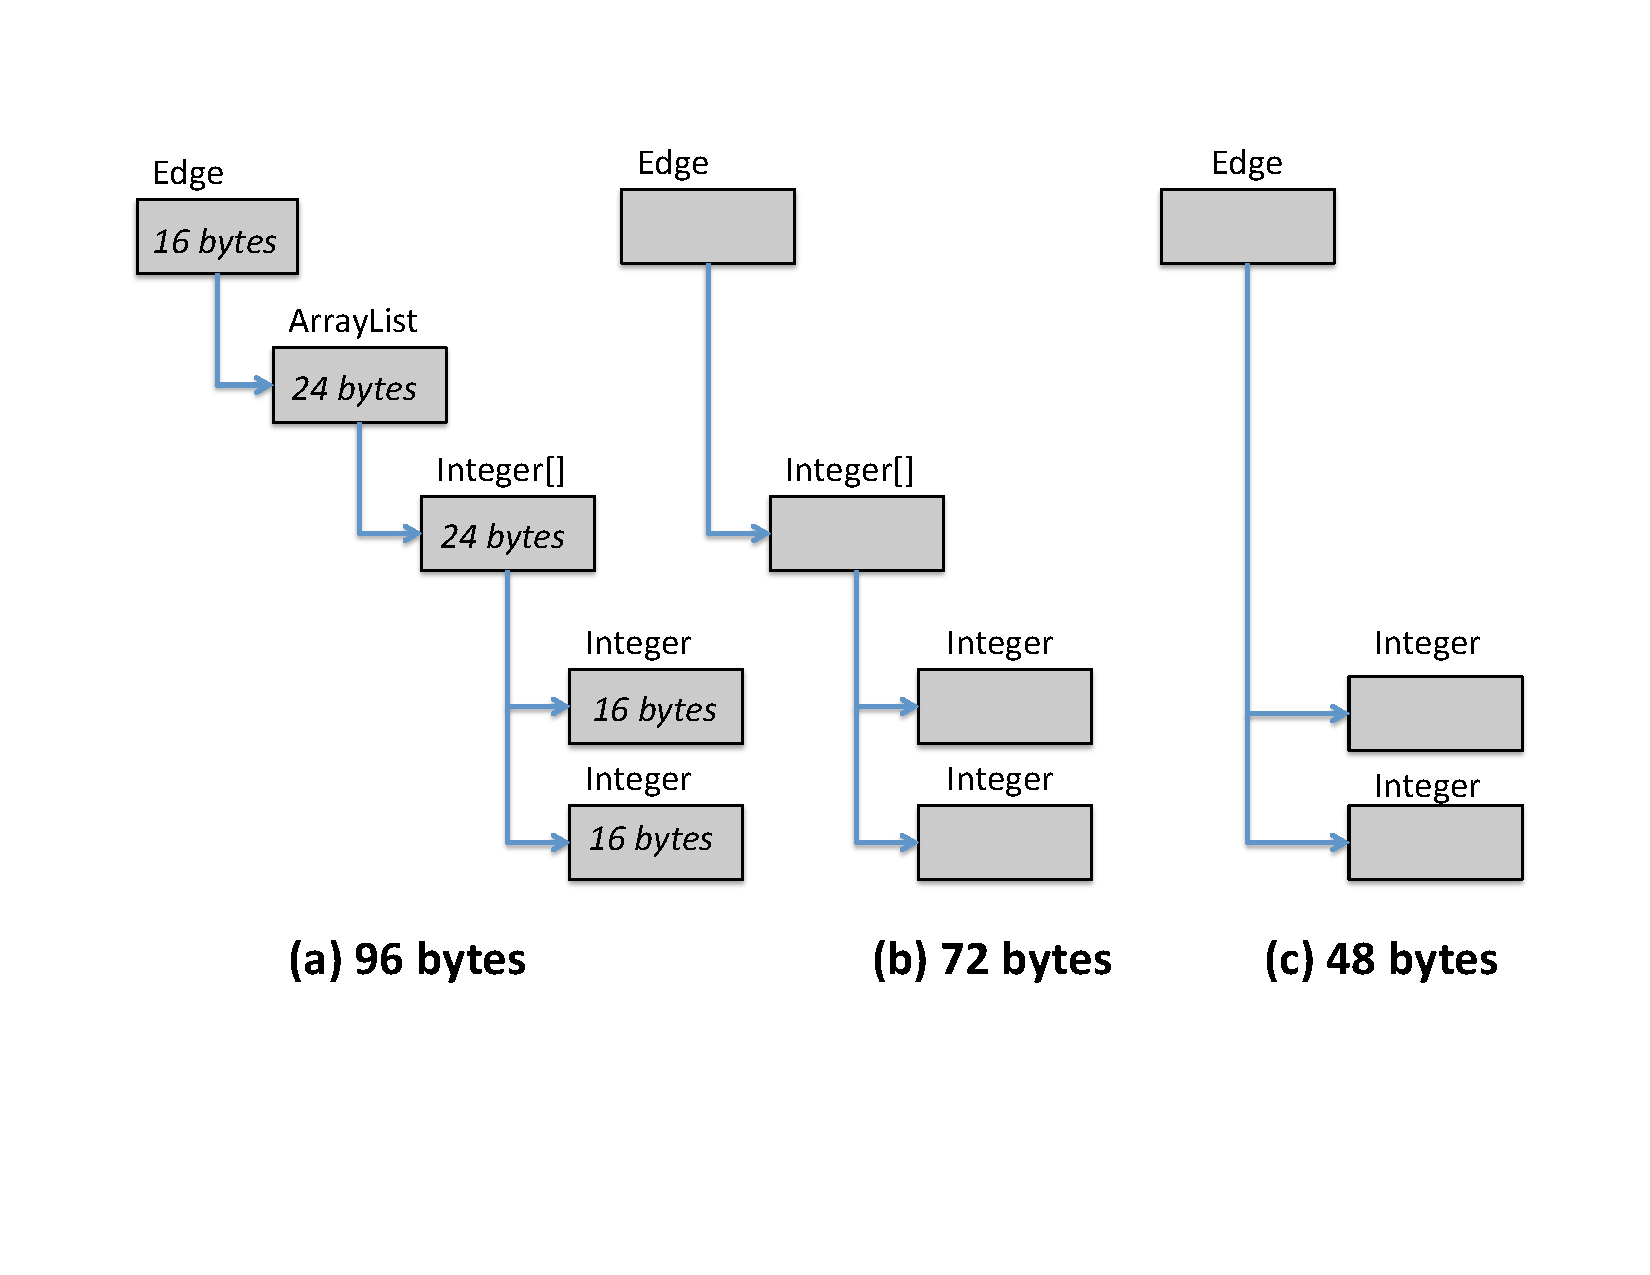
\includegraphics[width=.80\textwidth]{part1/Figures/collections/Edges.pdf}
%  \caption{(a) An \class{Edge} has 96 bytes. (b) Replacing the
%  \class{ArrayList} by an array eliminates 24 bytes. (c) Inlining the array
%  eliminates another 24 bytes.}
%  \label{fig:edges}
%\end{figure}
%This is an example of choosing an overly-general collection. In
%this situation, you don't need a collection at all. Using \class{ArrayList}
%for storing fixed- or bounded-size arrays is a
%common practice that can be easily avoided.
%
%There is one final optimization that can be performed on the \class{Product}
%class. Namely, making the four alternate suppliers into fields of
%\class{Product} instead of elements of an array. This optimization
% a 32 byte array object for 75,000 products, while adding three additional
% fields to the \class{Product} for 100,000 objects, saving another 1.1MB in
% total:
%\begin{shortlisting}
%class Product {
%	String sku;
%	String name;
%	.. 
%	Supplier alternateSupplier1;
%	Supplier alternateSupplier2;
%	Supplier alternateSupplier3;
%	Supplier alternateSupplier4;
%}
%\end{shortlisting}
%
%This representation is very similiar to the original \class{Product} class in
%section~\ref{sec:rarely-used} where there is one alternate suppler field, and
%here there are four. Taking all of the optimizations 
%together, we have gone from the initial \class{HashSet} representation
%of 22.1MB in Section~\ref{section:choosing-collection} to the in-lined field
%representation of 1.86MB. 


\section{Hybrid Representations}
\label{sec:hybrid-representations}
\subsection{Mostly-small collections}
\label{sec:mostly-small-collections}
It is often the case that the collections used in a relationship
are not of uniform size. There often are many collections that are small and fewer that are
very big.  It's reasonable to use an expensive collection like \class{HashSet}
for the big collections, but then the small collections pay the price. One way
to handle this problem is to use a hybrid representation. For example, you can
use \class{ArrayList}s for smaller collections, and \class{HashSet}s for larger
collections. 

One catch is that you usually will not know in advance which collections in the
relationship will end up being small and which will grow to be large. Therefore
one or more conversion operations will be necessary at some point if a
collection grows large enough. 

Returning to our original example, let's suppose that our average of 4 alternate
suppliers per product is distributed as follows: 25\% of products have no
alternate suppliers, 25\% have one alternate supplier, the next 25\% have
between 2 and 6, averaging 3 each, and the remaining 25\% have an
average of 12 each.
Let's also assume that we do in fact need to guarantee uniqueness in the data
model. The code for the \class{Product} class is shown below. As in the case of
lazy allocation, we'll need to hide access to the collections behind
accessor and update methods. 

\begin{shortlisting} 
public class Product {

	// Threshold for switching to HashSet
	private static final int arrayListMax = 6;
	.. 
	protected Collection<Supplier> alternateSuppliers;
	..
	public Product() {
		..
		// Initialize to a shared, empty collection
		alternateSuppliers = Collections.emptyList();
		..
	}
	
	public void addAlternateSupplier(Supplier supplier) {
		int numSuppliers = alternateSuppliers.size();
		if (numSuppliers == 0) {
			// Create a singleton list
			alternateSuppliers = 
				Collections.singletonList(supplier);
			return;
		}
		if (!(alternateSuppliers instanceof HashSet)) {
			// Uniqueness check for non-HashSet cases
			if (alternateSuppliers.contains(supplier)) {
				return;
			}
			if (numSuppliers == 1 && 
			 	!(alternateSuppliers instanceof ArrayList)) {
			 	// Convert to ArrayList
			 	alternateSuppliers = 
			 		new ArrayList<Supplier>(alternateSuppliers);
			}
			else if (numSuppliers == arrayListMax) {
				// Convert to HashSet
			 	alternateSuppliers = 
			 		new HashSet<Supplier>(alternateSuppliers);
			}
		}
		// Add supplier
		alternateSuppliers.add(supplier);
	}
	..
}
\end{shortlisting}

\paragraph{Singleton collections}
The standard library class \class{Collections} provides
\emph{singleton collections} that hold one element each.
These use much
less memory than their more general counterparts.
A singleton list and set take only 16 bytes each. Singleton collections
can be created via factory methods in \class{Collections}. In our
example, we first initialize the relationship with a shared
reference to a static empty set, in case there are no alternate suppliers. The method
\code{addAlternateSupplier} creates a singleton set to hold the first alternate supplier, if one is added. 
The singleton collections are immutable, in other words, they cannot be modified once they are
initialized. In your application, though, if you expect there to be
deletions and they are infrequent, it's easy enough to write code that simply
deletes the singleton collection until it's needed again.

\paragraph{Converting to larger representations}
If an additional alternate supplier is added, \code{addAlternateSupplier}
replaces the singleton list with an \class{ArrayList}. We can choose a
threshhold, say six entries, to be the maximum number of alternate
suppliers the \class{ArrayList} representation should hold.  If more
alternate suppliers are added beyond that, the representation is switched
to the more costly \class{HashSet}.
For the singleton and \class{ArrayList} representations, we need to check
uniqueness, and we use the \code{contains} method to do so. For \class{HashSet},
we can rely instead on
\class{HashSet}'s built-in uniqueness checking. 

%The method \code{addAlternateSupplier} adds the supplier to the array if the
%size is less than the threshold, otherwise, it adds the supplier to the
% \class{HashSet}.
%It allocates the alternate supplier array and \class{HashSet} 
%only if and when it is needed, to avoid wasting space with empty collections
%when there are no or only a few alternate suppliers.

Implementing hybrid representations is more complicated than just using one
type of collection for a relationship. However, it can save significant space in some
cases. In our example, an implementation that uses a
\code{HashSet} (minimally sized) and shares a single empty collection would
spend 18.9MB on collections overhead. The hybrid representation would reduce
that to 11.6MB, a 38\% savings. 
%This can save even more space.

\subsection{Load vs. use scenarios}
\label{sec:load-vs-use}

Another scenario where you can benefit from multiple representations is when you
have a distinct load phase followed by a phase where you only need read access
to the data. If your application requires more expensive functionality at load
time, such as uniqueness checking, frequent deletions, or maintenance of
insertion order, and you can afford a higher footprint during that phase, a
representation such as \class{HashSet} or \class{LinkedList} can be a simple
solution. Once loading is complete, you can make a second pass over
the data and replace the relationship with a more compact collection, such
as \code{ArrayList}. Since the cardinality of each collection is known in
advance, it is easy to allocate each \code{ArrayList} to the right size.

Depending on how much extra coding and maintenance you are willing to do, you
can further optimize by using arrays rather than collections, since you know the
size of each array in advance. This can save you
the cost of the \code{ArrayList} wrapper, or 24 bytes per collection. In
general we do not encourage coding your own collection functionality unless
you absolutely have to.  Most of the complexity of collection
behavior is in the update functionality, however. These collections are
readonly, which should make coding simpler.

Another alternative, if you would like to guarantee that the use-time
collections are readonly, is to use an immutable collection class, such as
one from the Guava open source framework. See
\autoref{sec:immutable-collections} for details.

The fastutil open source framework provides one more
solution for certain cases. Its \code{ObjectArraySet} class is one of the few
collection classes from any framework that uses less memory than the standard \code{ArrayList}.  Its
fixed cost is 32 bytes vs. the \code{ArrayList}'s 40.  It provides set behavior
backed by a simple array. Its only caveat is that its \code{contains} function
uses a linear search, which will be slow for a large set. 

\section{Special-purpose Collections}
\label{sec:special-purpose-collections}
Relationships sometimes have additional requirements,
such as synchronization or readonly behavior. In some cases, choosing a
special-purpose collection for the relationship will also result in a space
savings.
%For example, this is the case with singleton collections. 
In other instances,
however, collections with specialized functionality, even those that restrict functionality, 
can have hidden costs compared to their more
general counterparts. They may work fine as large
collections, but do not scale well when there are
many small collections, due to higher fixed costs.
In this section we look at a sampling of special-purpose
collections, and see how they work in the context of
relationships. \autoref{tab:specialized-collections-small} shows
the memory costs of the special-purpose collections discussed in this chapter.

\subsection{Immutable behavior}
\label{sec:immutable-collections}
The Guava open source framework includes a set of \emph{immutable} collection
classes.  They supply the same functionality as some of the 
common standard collections, but prevent update operations from being
performed. This can be useful if you have a relationship that
has distinct load and use phases, and you want to
guarantee at run time that there are no inadvertent
updates, once loading is complete. At the end of loading, simply switch the
representation to an immutable collection, as discussed in the previous
section. In some applications, the contents of each relationship instance will
even be known at load time, and remain constant thereafter. In
these cases you can allocate an immutable collection right from the start.

The class \code{ImmutableList} has the same fixed
and variable costs as the standard \code{ArrayList}, providing the
added protection at no additional cost.  If you require set functionality,
Guava provides an \code{ImmutableSet} class. It costs more than an
\code{ArrayList}, but considerably less than a \code{HashSet}.
For example, with 4 elements, its total overhead is 96 bytes, compared with
a \code{HashSet}'s 200. If you are willing to trade a
hash-based element lookup for a binary search, Guava's \code{ImmutableSortedSet} provides
further savings, giving you set functionality for the same memory cost as an
\code{ArrayList}.

\subsection{Unmodifiable behavior}
\label{sec:unmodifiable-collections}
Suppose our developer would like to allow users of the
data model to pass around the list of alternate suppliers for each product, 
but in a way that prevents inadvertent updates. A seemingly simple approach is
to implement the relationship with a collection that has \emph{unmodifiable}
behavior, and expose this reference as part of the data model's API. 

In the standard Java libraries, certain features such as
unmodifiable are provided by wrapping an existing collection with a
view that augments or restricts the behavior of the
underlying collection. The \code{Collections} class provides static factory
methods for this purpose. In contrast to an
immutable collection, whose contents will not change, an unmodifiable collection
is a view over a collection which may continue to change. 
The view may be passed to selected users to give them restricted access to the
underlying collection. Below is the code
to create unmodifiable \class{ArrayList}s in the data model:
 
\begin{shortlisting}
public class Product {
	..
	List<Supplier> alternateSuppliers;
	..
	public Product() {
		alternateSuppliers = Collections.unmodifiableList(new ArrayList());
		..
	}
	
}
\end{shortlisting}


\autoref{fig:product-unmodifiable-arraylist}
shows the E-C diagram when we add the unmodifiable behavior to our solution
from \autoref{fig:trimmed-product} in \autoref{sec:proper-size}, using
minimally-sized \class{ArrayList}s. The cost of the collections
increases from 5.3MB to 6.9 MB, or a 28\% increase in collection overhead.  The
inset shows why: each instance of the relationship now incurs an additional
fixed cost, that of the view wrapper.

It bears asking whether this feature, which serves a development-time
safety-checking purpose, is worth the relatively high run-time cost that results
when applying it at such a fine scale.  Alternative solutions are to encapsulate access to the
relationship, or to turn on the unmodifiable behavior only during testing.

\begin{figure}
  \centering
 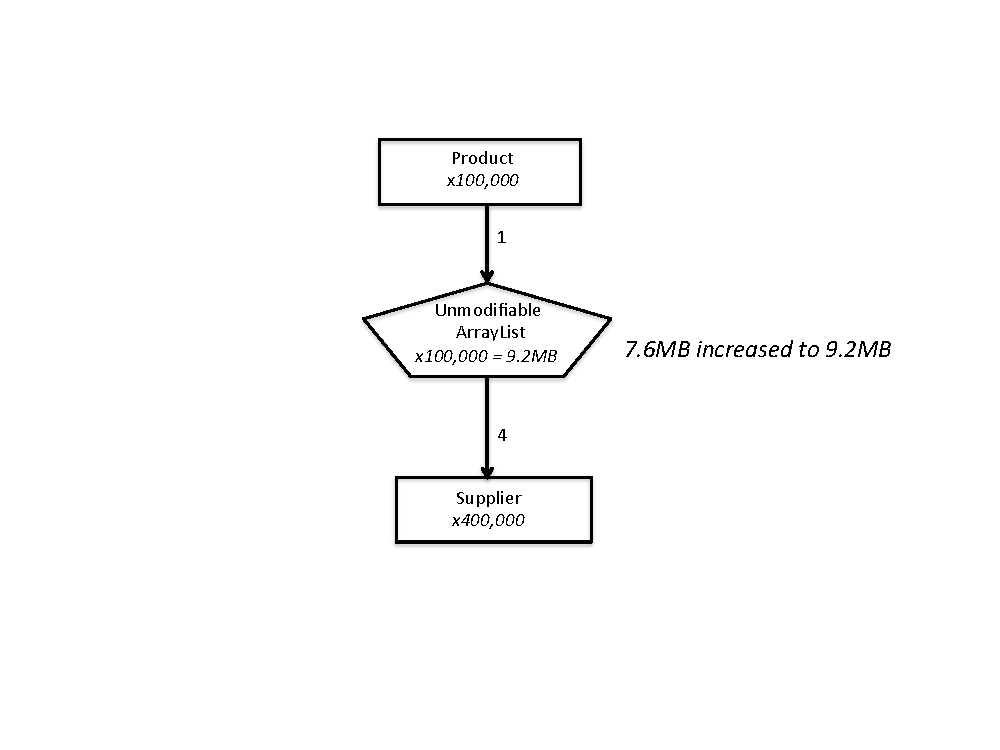
\includegraphics[width=.80\textwidth]{part1/Figures/collections/product-unmodifiable-arraylist.pdf}
 \caption{A relationship between 100,000 products and alternate suppliers,
 where the alternate \class{Supplier}s associated with each
 \class{Product} are stored in an \class{Unmodifiable ArrayList}. The inset
 shows how each collection now incurs the fixed cost of an additional
 view layer.}
  \label{fig:product-unmodifiable-arraylist}
\end{figure}



\subsection{Synchronized behavior}
\label{sec:synchronized-collections}
The standard Java collections, such as \code{ArrayList} and \code{HashSet}, do
not provide for synchronization. 
Java takes the same approach here as with unmodifiable behavior. To guarantee safe usage of a
collection from concurrent threads, you may create a synchronized view over it. 
Static factory methods from the \code{Collections} class are provided for this
purpose.

As with unmodifiable views, when using this feature for a relationship, the
view layer adds a fixed cost (see \autoref{tab:specialized-collections-small}) that will
be multiplied by the number of instances of the relationship. The memory cost
of using synchronized behavior at this scale can quickly add up. For a
relationship that will have infrequent accesses and updates from concurrent
threads, where latency is not an issue, adding synchronized behavior is a good
choice. It is a much less expensive choice than using
concurrent collections in this context\footnote{In the next chapter
we'll look at a more extreme example, of using concurrent collections at a fine granularity, at a huge memory cost.}.

The original Java 1 collections were written
with synchronized behavior built in. The Java 2 framework moved
this behavior out of the collections proper.
The older collections are still available, and are a less
expensive solution in some cases. There are some slight differences in
functionality.  At the same time, they have been updated to be compatible
with the Java 2 collections interfaces and with generics. The
\code{Vector} class provides for synchronization with fixed and variable costs
identical to those of the newer \code{ArrayList}.
\class{Hashtable} has similar costs to \class{HashMap}, but with a
smaller default capacity and more flexibility in setting the
initial capacity. There is no Java 1 analogue to \code{HashSet} or
\code{LinkedList}.


\begin{table}
\centering
 		\begin{tabular}{l||r||r||rrl}
 		\toprule
	 	 Collection & with 1 entry & with 4 entries &
	 	 \multicolumn{3}{c}{with n entries}\\
	 	 & & & fixed & variable & comments \\
	 	 \midrule
	 	\multicolumn{5}{l}{Collections statics:} \\
	 	\midrule
	 	SingletonSet &  16 & - & 16 & - &  \\
	 	SingletonList & 16 & - & 16 & - &  \\
	 	SingletonMap &  40 & - & 40 & - &  \\
	 	\midrule
	 	UnmodifiableList & - & - & 16 & - & add'l cost \\
	 	UnmodifiableSet & - & - & 16 & - & add'l cost \\
	 	UnmodifiableMap & - & - & 24 \footnotemark[3] & - & add'l cost \\
	 	\midrule
	 	SynchronizedList & - & - & 24  & - & add'l cost \\	 	
	 	SynchronizedSet & - & - & 16  & - & add'l cost \\	 	
	 	SynchronizedMap & - & - & 32 \footnotemark[4] & - & add'l cost \\	 	
	 	\midrule
	 	\multicolumn{5}{l}{Guava:} \\
	 	\midrule
	 	ImmutableList & 40 & 56 & 36 \footnotemark[1] & 4 & for any n \\
	 	ImmutableSet & 64 & 96 & 64 \footnotemark[2] & 8 & for any n \\
	 	ImmutableSortedSet & 40 & 56 & 36 \footnotemark[1] & 4 & for any n \\
	 	 \midrule
	 	\multicolumn{5}{l}{fastutil:} \\
	 	\midrule
	 	ObjectArraySet & 32 & 48 & 28 \footnotemark[1] & 4
	 	& for any n \\
	 	\midrule
	 	\multicolumn{5}{l}{Java 1 collections:} \\
	 	\midrule
	 	Vector & 40 & 56 & 36 \footnotemark[1]  & 4 & for any n\\ 	
	 	\bottomrule
	 	\end{tabular}
	 	
	\caption{A sampling of special-purpose collections and their costs. Assumes
	minimally-sized collections, when applicable.}
	\label{tab:specialized-collections-small}
\end{table}

\footnotetext[1]{Round total cost up to nearest 8 bytes.}
\footnotetext[2]{Round total cost up to nearest 16 bytes.}
\footnotetext[3]{There is an additional fixed cost if you iterate over the keys
or values (not the entries). An unmodifiable view is created over the key set or
values collection, and will persist for the lifetime of the original
collection.} 
\footnotetext[4]{There is an additional fixed cost if you iterate over the keys,
entries, or values. A synchronized view is created over the key set,
entry set, or values collection, and will persist for the lifetime of the
original collection.}

\FloatBarrier

\section{Summary}

When collections are used to represent relationships, they often result in many
small collection instances. Their cost is dominated by fixed-size
overhead; variable overhead matters as well. To mitigate high memory costs
for relationships:
%implemented with collections:
\begin{itemize}
  \item Choose the most memory-efficient collection for the job at hand. For
  example, when collections have at most a few elements in them, you
  don't need expensive functionality like hashing. In
  order to choose, first ask some questions about the relationship:
  \begin{itemize}
    \item What operations will be performed? Will there be deletions,
    insertions, uniqueness checks?
    \item What's the expected cardinality? Is it uniformly
    distributed, or will there be mostly small
    collections and a few large ones? Will there be many empty collections?
    \item Is there a distinct load phase, after which the relationship no
    longer changes?
  \end{itemize}
  \item Make sure collections are properly sized. If you know that a collection
  will not grow any more, then there is no reason to maintain extra room for
  growth.
  \item Avoid lots of empty collections. You can postpone creating collections
  until they are needed.
 \item When the size distribution is not uniform, it is sometimes reasonable to
 use a hybrid representation that adapts to the data. If there are
 distinct load vs. use phases, a different representation
 for each phase can sometimes be a good solution.
 \item Some special-purpose collections can help save space, such as
 \code{SingletonSet}. Others are not
 designed for use at a small scale. Make sure the
 behavior is worth the added cost.
\end{itemize}
Knowing which relationships and collections in your application are the most
important and need to scale is key to applying these optimizations effectively.  




